\documentclass{homework}
\usepackage{ctex, bm}
\usepackage{makecell}
\usepackage[ruled,vlined]{algorithm2e}
\usepackage{booktabs}
\usepackage{multirow}
\usepackage{siunitx}
\usepackage{graphicx}
\usepackage{amsmath}
\usepackage{subcaption}
\usepackage{caption}
\newcommand{\bfx}{\mathbf{x}}
\newcommand{\bfg}{\mathbf{g}}
\newcommand{\bfH}{\mathbf{H}}
\newcommand{\bfd}{\mathbf{d}}
\author{李健宁}
\class{机器学习中的优化问题}
\date{\today}
\title{Homework 12}
% \address{Bayt El-Hikmah}

\graphicspath{{./media/}}

\begin{document} \maketitle

\question

\begin{sol}
    $\nabla f(x) = 2\mathbf{D}^\top (\mathbf{D}\bfx - \mathbf{y})$,限制条件为$\|\cdot\|_1$时,
    \[
    \mathbf{s}_k = \arg\min_{\mathbf{s}\in \mathbf{D}}\langle\mathbf{s},\mathrm{\textbf{g}}\rangle = -\text{sign}(g_i)\mathbf{\textbf{e}}_i, \, i = \arg\max_j |g_j|.
    \]
    限制条件为$\|\cdot\|_\infty$时,
    \[
    \mathbf{s}_k = \arg\min_{\mathbf{s}\in \mathbf{D}}\langle\mathbf{s},\mathrm{\textbf{g}}\rangle = -\text{sign}(\mathrm {\textbf{g}}).
    \]
    设向量 $\mathbf{v} \in \mathbb{R}^n$,投影到 $\ell_1$ 范数球上的问题是
\[
\min_{\mathbf{x}} \|\mathbf{x} - \mathbf{v}\|_2^2 \quad \text{s.t.} \quad \|\mathbf{x}\|_1 \leq \tau,
\]
这个问题的解是
\[
x_i = \mathrm{sign}(v_i) \cdot \max\left(|v_i| - \theta, 0\right)
\]

 $\theta$ 通过以下步骤计算:
\begin{enumerate}
  \item 令 $u = \mathrm{sort}(|\mathbf{v}|)$,按降序排列。
  \item 计算累计和 $S_k = \sum_{j=1}^{k} u_j$。
  \item 找到最大的 $\rho$ 满足$  u_\rho > \frac{1}{\rho} \left(S_\rho - \tau \right)$
  \item $\theta = \frac{1}{\rho} \left(S_\rho - \tau\right)
  $
\end{enumerate}

投影梯度法选择固定步长$\alpha = 0.0001$,$f^*$通过运行5000次两个方法比较较小值获得,实验中分别迭代两种方法$2000$次,实验结果如图\ref{1},能够看出投影梯度法无论是收敛速度还是稳定性上都更占据优势。
\begin{figure}[h]
    \centering
    \begin{subfigure}[t]{0.48\textwidth}
        \centering
        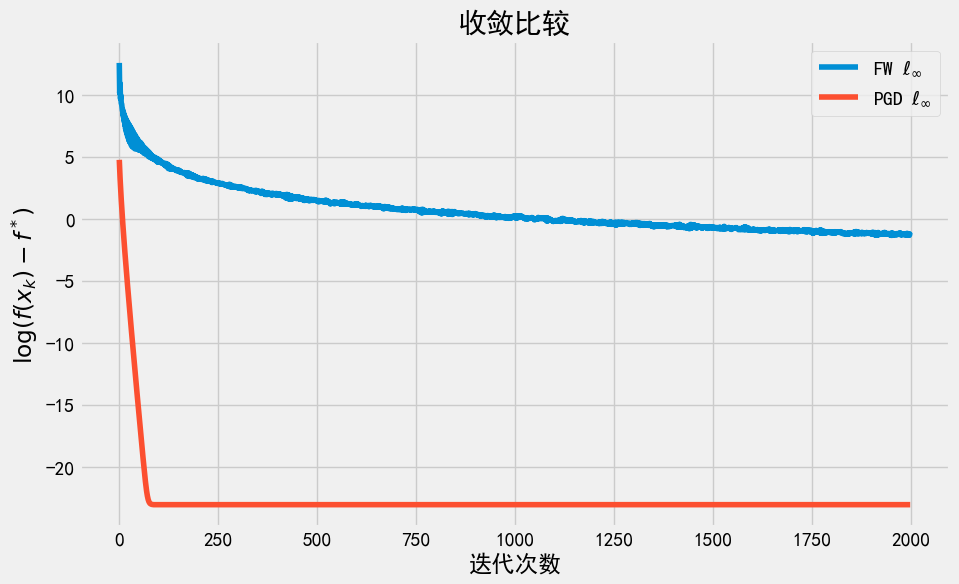
\includegraphics[width=\linewidth]{1.png}
        \caption{$\ell_\infty$范数}
    \end{subfigure}
    \hfill % 添加一些水平间距
    \begin{subfigure}[t]{0.48\textwidth}
        \centering
        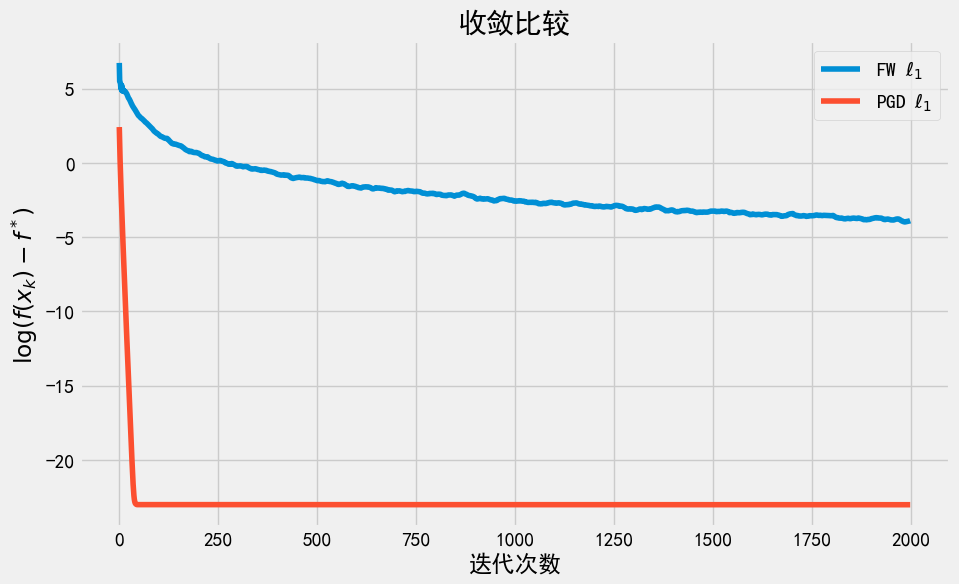
\includegraphics[width=\linewidth]{2.png}
        \caption{$\ell_1$范数}
    \end{subfigure}
    \caption{收敛速度对比}\label{1}
\end{figure}

\end{sol}

\question

\begin{sol}

    \[
    \min_{\mathbf{x}, \mathbf{y}} f(\mathbf{x}) + g(\mathbf{y}) \quad \text{s.t.} \quad \mathbf{x} = \mathbf{y}
    \]
    
    其中:
    \[
    f(\mathbf{x}) = \|\mathbf{x} - \mathbf{a}\|_2, \quad g(\mathbf{y}) = \|\mathbf{y} - \mathbf{b}\|_1, \quad \mathbf{a} \neq \mathbf{b} \in \mathbb{R}^{100}
    \]
    
    \subsection*{Dual Ascent 方法推导}
    
    拉格朗日函数为:
    \[
    \mathcal{L}(\mathbf{x}, \mathbf{y}, \boldsymbol{\lambda}) = f(\mathbf{x}) + g(\mathbf{y}) + \boldsymbol{\lambda}^\top (\mathbf{x} - \mathbf{y})
    \]
    
    对偶函数为:
    \[
    d(\boldsymbol{\lambda}) = \inf_{\mathbf{x}} \left( f(\mathbf{x}) + \boldsymbol{\lambda}^\top \mathbf{x} \right) + \inf_{\mathbf{y}} \left( g(\mathbf{y}) - \boldsymbol{\lambda}^\top \mathbf{y} \right)
    \]
    
    Dual Ascent 迭代更新如下:
    \[
    \begin{aligned}
    \mathbf{x}^{k} &= \arg\min_{\mathbf{x}} f(\mathbf{x}) + \boldsymbol{\lambda}^k{}^\top \mathbf{x} \\
    \mathbf{y}^{k} &= \arg\min_{\mathbf{y}} g(\mathbf{y}) - \boldsymbol{\lambda}^k{}^\top \mathbf{y} \\
    \boldsymbol{\lambda}^{k+1} &= \boldsymbol{\lambda}^k + \eta (\mathbf{x}^k - \mathbf{y}^k)
    \end{aligned}
    \]
    可以求出
    \[
\begin{aligned}
    \mathbf{x}^{k+1} &= \mathbf{a} - \operatorname{proj}_{\mathcal{B}_2(1)}(\boldsymbol{\lambda}^k)
= \mathbf{a} - \boldsymbol{\lambda}^k \cdot \min\left(1, \frac{1}{\|\boldsymbol{\lambda}^k\|_2}\right)\\
\mathbf{y}^{k+1} &= \mathbf{b} - \operatorname{clip}(\boldsymbol{\lambda}^k, -1, 1, -1, 1)
\end{aligned}
\]
    \subsection*{ADMM 方法推导}
    
    增广拉格朗日函数为:
    \[
    \mathcal{L}_{\beta}(\mathbf{x}, \mathbf{y}, \boldsymbol{\lambda}) = f(\mathbf{x}) + g(\mathbf{y}) + \boldsymbol{\lambda}^\top (\mathbf{x} - \mathbf{y}) + \frac{\beta}{2} \|\mathbf{x} - \mathbf{y}\|_2^2
    \]
    
 定义
    \[
    \mathbf{u}^k = \frac{1}{\beta} \boldsymbol{\lambda}^k
    \]
    
    ADMM 的迭代更新步骤如下:
    \[
    \begin{aligned}
    \mathbf{x}^{k+1} &= \arg\min_{\mathbf{x}} f(\mathbf{x}) + \frac{\tau \beta}{2} \|\mathbf{x} - \mathbf{y}^k + \mathbf{u}^k\|_2^2 \\
    \mathbf{y}^{k+1} &= \arg\min_{\mathbf{y}} g(\mathbf{y}) + \frac{\tau \beta}{2} \|\mathbf{x}^{k+1} - \mathbf{y} + \mathbf{u}^k\|_2^2 \\
    \mathbf{u}^{k+1} &= \mathbf{u}^k + \mathbf{x}^{k+1} - \mathbf{y}^{k+1}
    \end{aligned}
    \]
    可以求出
    \[
\begin{aligned}
\mathbf{x}^{k+1} &= \mathbf{a} + \max\left(1 - \frac{1}{\tau\beta \|\mathbf{z} - \mathbf{a}\|_2}, 0\right) (\mathbf{a} - \mathbf{z}),\, \mathbf{z}= \mathbf{y}^k - \mathbf{u}^k\\
\mathbf{y}^{k+1} &= \operatorname{soft}_{1/(\tau\beta)}(\mathbf{v} - \mathbf{b}) + \mathbf{b},\,\mathbf{v} = \mathbf{x}^{k+1} + \mathbf{u}^k
\end{aligned}\]
其中
\[
\operatorname{soft}_\lambda(z_i) = \operatorname{sign}(z_i) \cdot \max(|z_i| - \lambda, 0).
\]

测试时,取ADMM的步长$\beta \in [1, 10, 100],\tau = [0.5, 1.0, 1.5]$,迭代次数均为$600$次。$f^*$通过运行3000次$\beta = 1,\tau = 0.5$获得。实验结果如图\ref{2},可以看出$\tau\beta$越小,收敛越快。
\begin{figure}[h]
    \centering
        \centering
        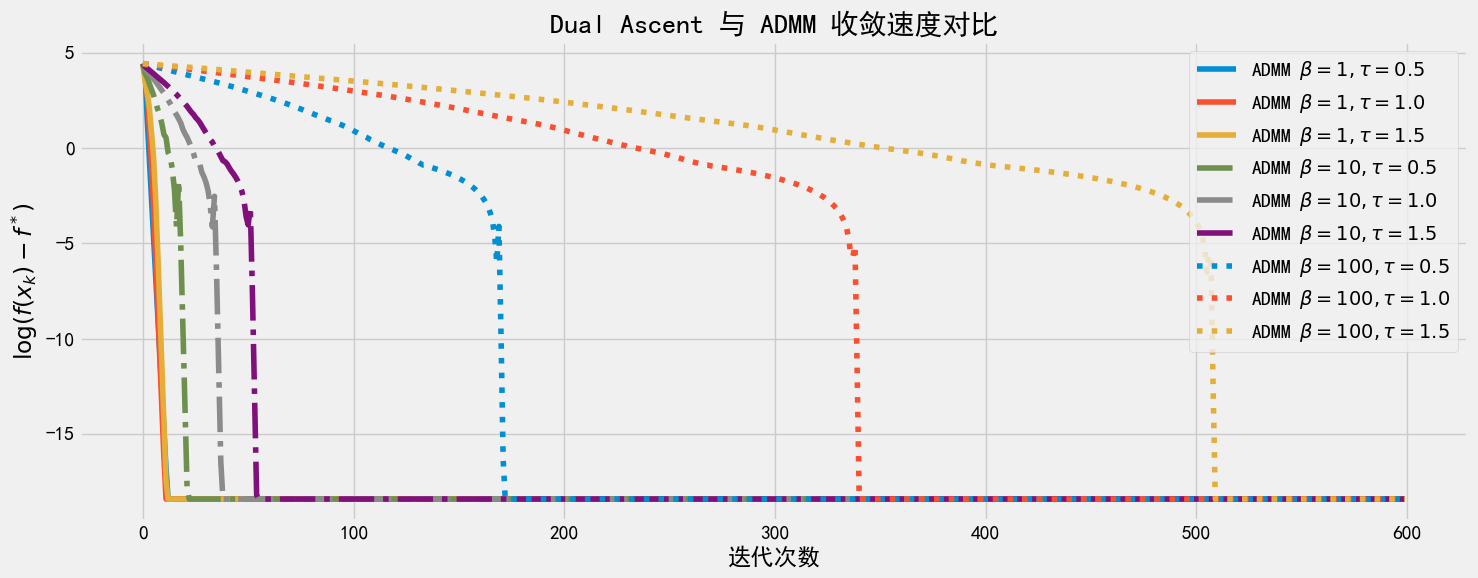
\includegraphics[width=0.8\linewidth]{3.png}
        \caption{ADMM收敛对比}\label{2}
\end{figure}

另外,Dual Ascent方法未能收敛,可能是因为$f(x)$和$g(y)$的性质不佳,$f(x)$非强凸,而$g(x)$不可导,导致Dual Ascent方法在迭代时可能会出现不收敛。

\end{sol}

\question

\begin{sol}
    引入拉格朗日乘子 \( Y_1 \in \mathbb{R}^{m \times n} \),\( Y_2 \in \mathbb{R}^{n \times 1} \),增广拉格朗日函数为:

\[
\begin{aligned}
\mathcal{L}(Z, E, Y_1, Y_2) = &\|Z\|_* + \lambda \|E\|_{2,1} + \langle Y_1, D - DZ - E \rangle + \frac{\beta}{2} \|D - DZ - E\|_F^2 \\
&+ \langle Y_2, Z^\top \mathbf{1} - \mathbf{1} \rangle + \frac{\beta}{2} \|Z^\top \mathbf{1} - \mathbf{1}\|_2^2
\end{aligned}
\]


\subsection*{更新 \( Z \)}

我们线性化增广拉格朗日中关于 \( Z \) 的二次项,得到以下更新:

\[
Z^{k+1} = \arg\min_Z \|Z\|_* + \frac{\beta_k}{2} \|Z - G^k\|_F^2
\]

其中:

\[
G^k = Z^k - \frac{1}{\eta_D} \left( D^\top (D Z^k + E^k - D) + \mathbf{1}(Z^{k\top} \mathbf{1} - \mathbf{1})^\top + \frac 1{\beta_k}D^\top Y_1^k + \frac 1{\beta_k}\mathbf{1} Y_2^{k^\top} \right)
\]

该子问题的解为奇异值软阈值:

\[
Z^{k+1} = \operatorname{SVT}_{1/\eta_D\beta_k}(G^k)
\]

\subsection*{更新 \( E \)}

对 \( E \) 的更新为:

\[
E^{k+1} = \arg\min_E \lambda \|E\|_{2,1} + \frac{\beta_k}{2} \left\| E - \left(D - D Z^{k+1} + \frac{1}{\beta_k} Y_1^k \right) \right\|_F^2
\]

这是 \( \ell_{2,1} \) 范数的近端问题,解为对每列进行缩放:

\[
E^{k+1}_{:,j} = \left[1 - \frac{1}{\beta_k\|R_{:,j}\|_2} \right]_+ R_{:,j}, \quad R = D - D Z^{k+1} + \frac{1}{\beta_k} Y_1^k
\]

\subsection*{更新拉格朗日乘子}

\[
\begin{aligned}
Y_1^{k+1} &= Y_1^k + \beta_k (D - D Z^{k+1} - E^{k+1}) \\
Y_2^{k+1} &= Y_2^k + \beta_k (Z^{k+1^\top} \mathbf{1} - \mathbf{1})
\end{aligned}
\]

\subsection*{自适应步长更新}

使用如下策略自适应更新 \( \beta_k \):

\[
\beta_{k+1} = \min(\rho \beta_k, \beta_{\max})
\]
$$
\rho= \begin{cases}\rho_0, & \text { if } \beta_k \max \left(\sqrt{\eta_D}\left\|\mathbf{x}_{k+1}-\mathbf{x}_k\right\|, \left\|\mathbf{y}_{k+1}-\mathbf{y}_k\right\|\right) /\|\mathbf{c}\|<\varepsilon_2 \\ 1, & \text { otherwise }\end{cases}
$$
\subsection*{收敛条件}
\[
\frac{\|DZ^k+E^k - D\|}{\|D\|}\le \epsilon_1,\, \text{or}
\max\left( \frac{\|D^k-D^{k-1}\|}{\|D\|}, \frac{\|E^k-E^{k-1}\|}{\|D\|} \right) < \epsilon_2
\]

\subsection*{数据实验}

参数选取上, \(\epsilon_1 = 10^{-6},\, \epsilon_2=10^{-5},\, \beta_0=\min(n,m)\epsilon_2 = 200\epsilon_2,\, \beta_{\max}=10^{10},\, \rho_0 = 1.9,\,\eta_D = 1.02\sigma^2_{\max}(\mathrm D) \),$\lambda = 0.1$,最大迭代次数5000次。最终实验结果如图\ref{4}
\begin{figure}[h]
    \centering
        \centering
        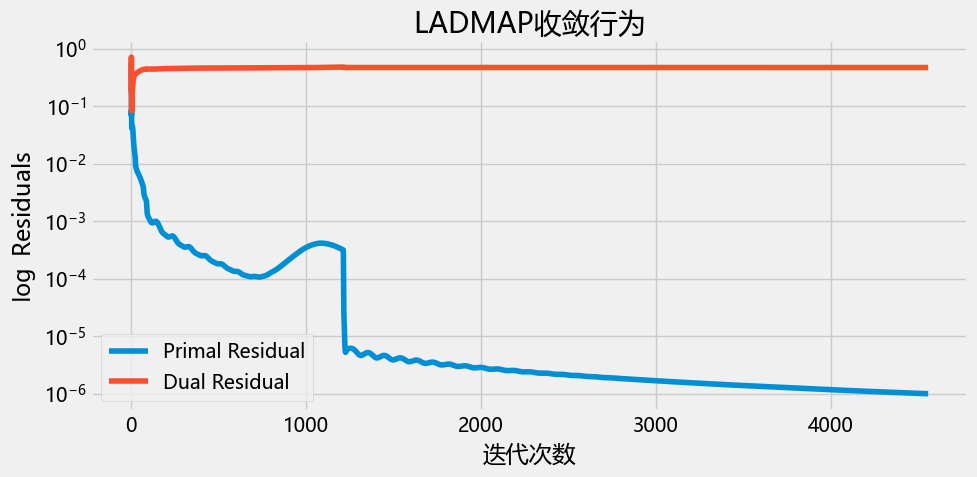
\includegraphics[width=0.8\linewidth]{4.png}
        \caption{LADMAP收敛行为}\label{4}
\end{figure}
\end{sol}

    % citations
% \bibliographystyle{plain}
% \bibliography{citations}

\end{document}
